\section{Erweiterte Partitionierung: Installationsziel w�hlen}
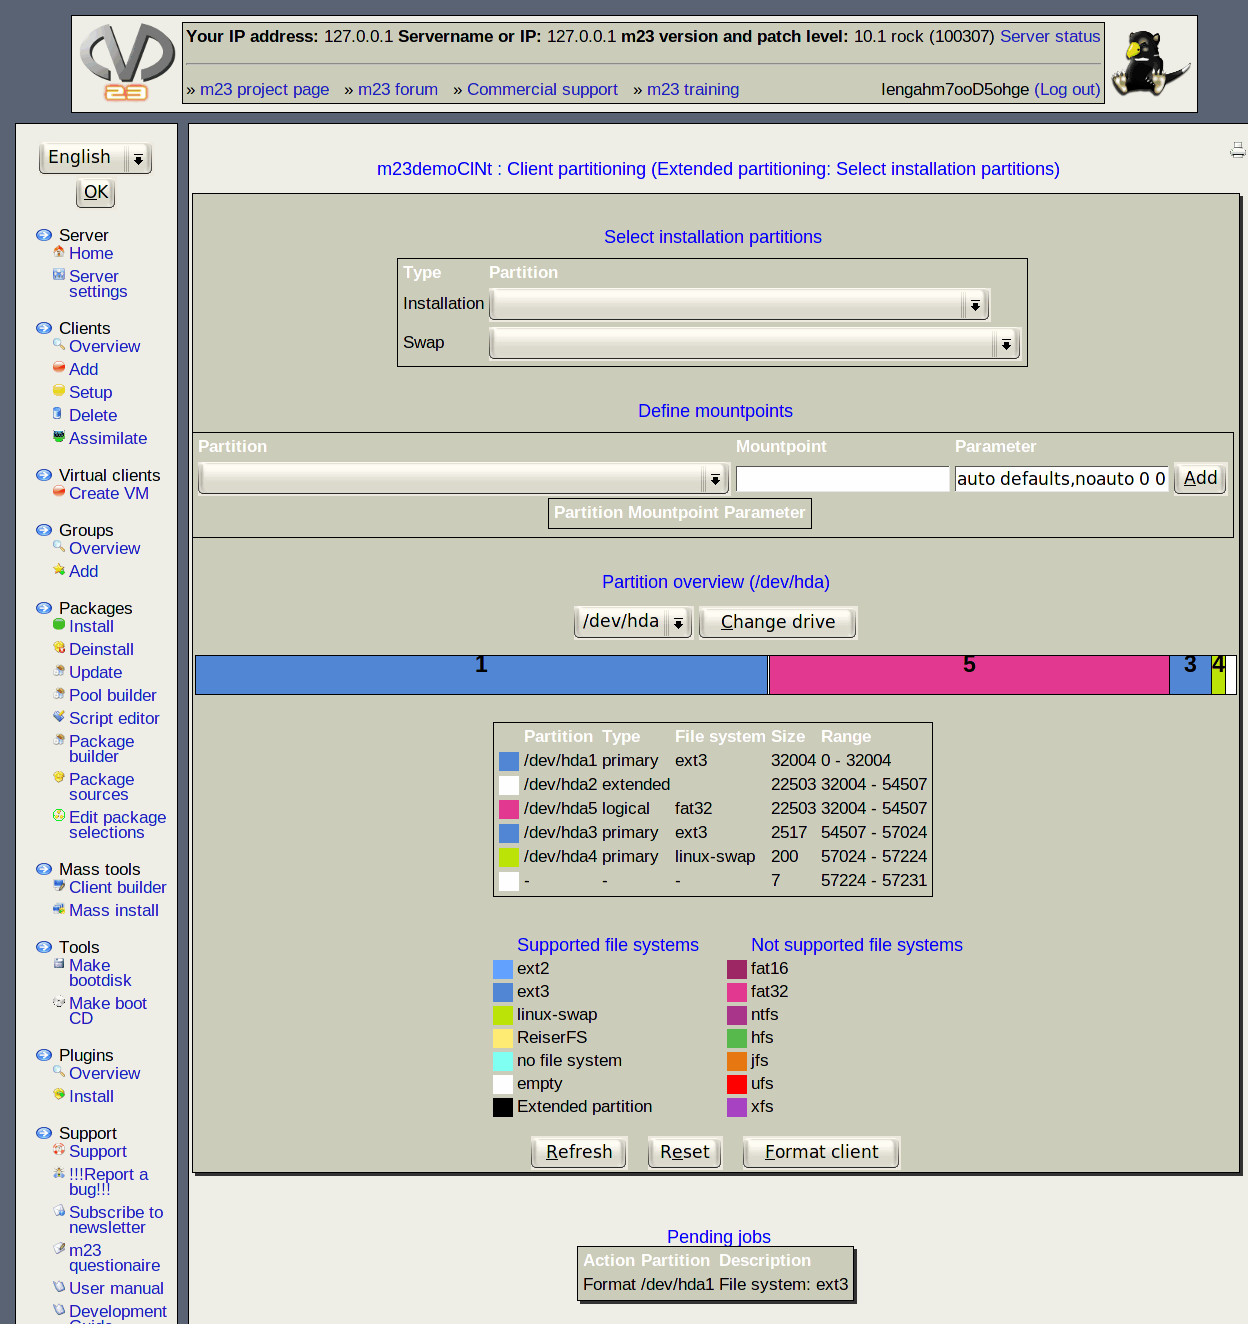
\includegraphics[scale=0.4]{/mdk/doc/manual/screenshots/de/fdisk-extended3.png} \\
W�hlen Sie die Partitionen aus, die Sie f�r die Installation nutzen m�chten. W�hlen Sie hierzu zwei Partitionen aus. Die erste, um das Betriebssystem zu installieren und die zweite als Auslagerungsplatz (Swap).\\
\subsection{Schrittweises Vorgehen:}
\begin{enumerate}
\item W�hlen Sie die Partitionen aus, die Sie zur Installation und als Swap nutzen m�chten.\\
\item Falls Sie zus�tzliche Mountpunkte ben�tigen, k�nnen Sie diese unter \textit{"Mountpunkte definieren"} erstellen. Geben Sie dazu die Partition, den Mountpunkt und zum Mounten ben�tigte Parameter an und klicken Sie anschlie�end auf \textit{"Hinzuf�gen"}. Diese Informationen entsprechen denen, die auf einem Linux-System in der Datei \textbf{/etc/fstab} stehen. In der Tabelle unter den Eingabefeldern k�nnen Sie die bereits definierten Mountpunkte sehen.\\
\item Klicken Sie auf \textit{"Client formatieren"}, um die Angaben zu �bernehmen\\
\end{enumerate}
\subsection{Hinweis zur Installation auf einem RAID}
Wie bereits in den vorherigen Hilfetexten angek�ndigt, m�ssen Sie einen extra Mountpunkt definieren, wenn Sie das Betriebssystem auf einem RAID installieren. Verwenden Sie hierzu eine Partition, die nicht auf einem RAID liegt und w�hlen Sie diese unter \textit{"Partition"} aus. Unter \textit{"Mountpunkt"} geben Sie bitte \textbf{"/boot"} und unter \textit{"Parameter"} \textbf{"auto defaults,noauto 0 0"} an.\\
